\begin{figure}[!htbp]
\centering
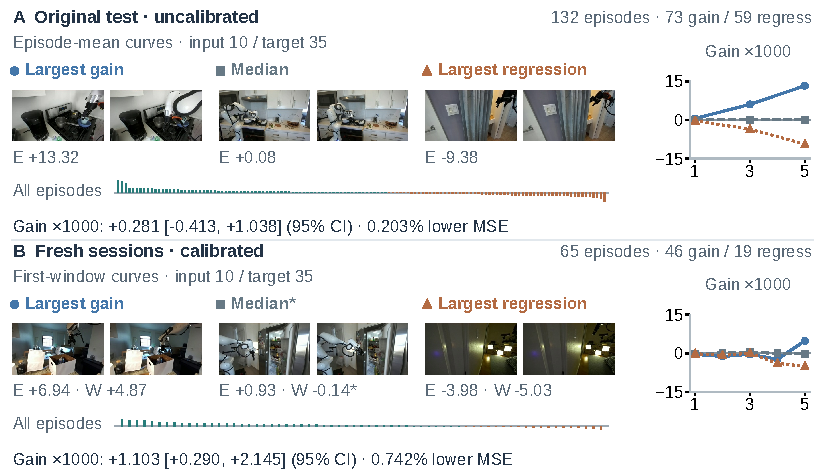
\includegraphics[width=\linewidth]{generated/editorial/recorded_forecast_compact.pdf}
\caption{\textbf{Matched recordings in two separate DROID studies of the historical context model (ours).} Each band retains the previously selected largest-gain, median and largest-regression episodes; selection is outcome-conditioned. Photos are complete recorded input/target frames 10/35 from the fixed first window, not predicted RGB. Gain is matched Framewise minus context-model standardized feature MSE; all MSE gains, curves, ranked marks and intervals are multiplied by 1,000. E/W denote episode/first-window h5 gains. Three-seed mean curves use all episode windows at h1/3/5 in (A), and the first window at h1--5 after matched train-fitted calibration in (B). *The fresh median episode improves while its shown window regresses. Each action block contains five recorded commands; connecting lines guide the eye. Ranked strips retain all 132/65 episodes. Population intervals are paired 95\% session/seed bootstraps; percentages compare population mean errors. Complete absolute method curves remain in the source pack; population values are in Tables~\ref{tab:real-video-primary} and~\ref{tab:fresh-real-video-complete}.}
\label{fig:real-video-comparison}
\label{fig:fresh-mechanism}
\end{figure}
